\section{Background}\label{sec:background}

% Curlie
Homepage2Vec~\cite{homepage2vec} is trained on the publicly available website directory called Curlie~\cite{curlie}. The directory comprises three million websites in 92 languages, labeled according to a taxonomy of hierarchical topics. The authors retain 886,000 websites and only consider the 14 top-level categories (see \ref{app:example-1-shot}). Multiple topics can be assigned to a single website - however, only 2.1\% of samples are actually labeled with more than one topic. The dataset is highly imbalanced, with the largest number of pages being categorised as Business (27\%) and the lowest as Kids and Teens (1.1\%). We will refer to this dataset as \texttt{curlie}.


% Architecture/ Training
Architecturally, Homepage2Vec is simple multi-layer perceptron (MLP) that uses embeddings of various website features as inputs.
Specifically, the model uses the \texttt{tld} (top-level domain), \texttt{domain}, \texttt{metatags}, \texttt{title}, \texttt{description}, \texttt{keywords}, \texttt{links}, and \texttt{sentences} as features. With the exception of \texttt{tld} and \texttt{metatags}, which are one-hot encoded, all features are embedded via the multilingual model XLM-R~\cite{xmlr} and finally concatenated. The resulting embedding is then through a two-layer MLP to produce a logit for each of the 14 categories. Importantly, each output logit is interpreted as the probability of a website belonging to a single category, allowing multilabel predictions. For details about the architecture and training procedure, please refer to the original paper~\cite{homepage2vec}. A simplified overview of the model architecture is part of Figure~\ref{fig:train-overview}.

% Evaluation
The original paper evaluates the model on the \texttt{curlie} dataset. Because of the unexhaustive labeling of websites, they additionally crowd-sourced annotations for 840 websites from the Curlie index. We will refer to this dataset as \texttt{crowdsourced}. As the authors do not report the exhaustive performance metrics on this data, we establish our own baseline. The baseline macro F1-score is $39.16\%$. 

\begin{figure}[!ht]
    \centering
    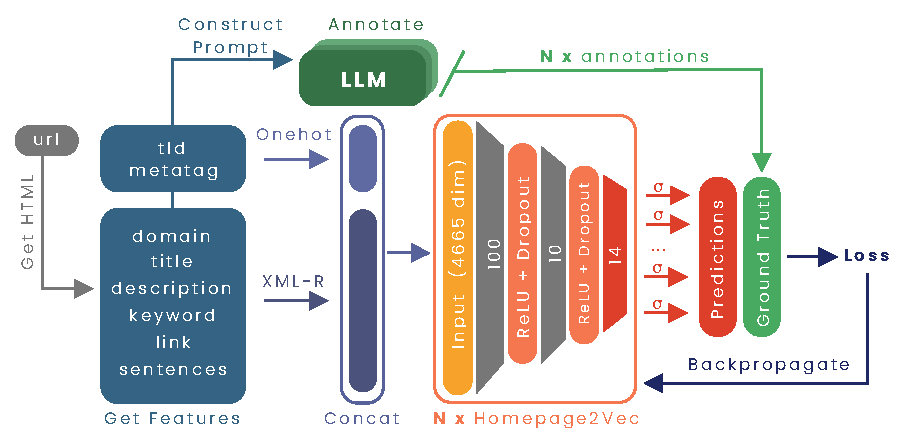
\includegraphics[height=0.2\textheight, width=\columnwidth]{./figures/training_overview.pdf}
    \caption{\textbf{Finetuning Overview.} The Figure depicts the finetuning procedure of Homepage2Vec. Various website features are extracted, embedded and fed into Homepage2Vec to produce predictions. Before, the processed website features are used to query a LLM labeler. The resulting labels are used to finetune Homepage2Vec.}
    \label{fig:train-overview}
\end{figure}

%$ \subsection{LLM Labeling}
%$ 
%$ Previous studies have demonstrated that LLMs are capable of executing various tasks without being specifically trained for them, especially when providing an informative prompt, a few examples, and a task description. This makes LLMs an attractive candidate to perform website classification directly by simply providing a set of features as input and ask the model to predict from a set of website categories.
%$ However, direct inference using LLMs is less practical due to their substantial cost and time demands during inference. A better approach is therefore to use LLMs to create a training dataset for a classifier, a technique known as \textit{knowledge distilation} and shown  effective in prior studies~\cite{reduce-labeling-cost, prompt-tuning, is-gpt3-good-annot, annollm}. Contrasting with earlier research that concentrated on single-label classification with limited categories, our research explores the quality of LLM-generated labels in a more complex scenario of multilabel classification across 14 website topics.
